W sekcji dotyczącej ustawień 3D dźwięków, skupiamy się na implementacji efektów przestrzennych, które pomagają uzyskać bardziej realistyczne doznania dźwiękowe w grze. W przypadku naszej gry, kontrola nad efektami przestrzennymi staje się istotna dla zwiększenia immersji gracza.

Przykłady sytuacji, w których kontrola 3D dźwięków może być kluczowa:

\begin{enumerate}
    \item \textbf{Dźwięk broni:} Podczas strzelania z broni, efekty przestrzenne pozwalają na dokładne odwzorowanie źródła dźwięku w zależności od kierunku, w którym strzelasz. To może poprawić orientację gracza w otoczeniu oraz dostarczyć dodatkowych wrażeń związanych z użytkowaniem broni.
    \item \textbf{Dźwięk granatów:} Efekty przestrzenne umożliwiają precyzyjne określenie pozycji, w której eksplodował granat oraz odległości od naszego miejsca. Gracz będzie w stanie lepiej zrozumieć, czy zagrożenie pochodzi z przodu, tyłu czy z boku, co może wpłynąć na jego taktykę.
    \begin{figure}[h]
            \centering
            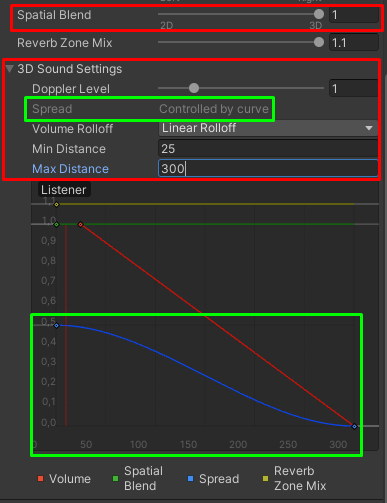
\includegraphics[scale=0.5]{Images/grenade3DSet.png}
            \caption{Przykładowe ustawienie 3D dźwięku dla obiektu granatu}
        \end{figure}
    \FloatBarrier
    W ustawieniach dźwięku 3D dla granatu, warto zwrócić uwagę na kilka kluczowych parametrów:
        \begin{itemize}
        \item \textbf{Spatial Blend:} Określa, jak bardzo dźwięk jest przestrzenny w stosunku do źródła. Wartość 1 oznacza, że dźwięk jest w pełni przestrzenny, natomiast wartość 0 oznacza, że dźwięk jest zupełnie dwuwymiarowy.
        \item \textbf{3D Sounds Settings:} Pozwala na dostosowanie wielu parametrów dźwięku przestrzennego, takich jak odległość, w jakiej dźwięk słychać, szybkość spadku głośności w zależności od odległości czy także szybkość przemieszczania się dźwięku.
        \item \textbf{Spread:} Określa rozproszenie dźwięku, czyli jak szeroko dźwięk jest rozprzestrzeniony w przestrzeni. Wartość 0 oznacza brak rozproszenia, a wartość 360 oznacza pełne rozproszenie wokół źródła dźwięku.
        \end{itemize}
    \item \textbf{Dźwięk otwieranych skrzynek:} Kontrola 3D dźwięków może pomóc w tworzeniu bardziej realistycznego doświadczenia podczas otwierania skrzynek czy innych kontenerów. Dźwięk tych elementów będzie można precyzyjnie zlokalizować w przestrzeni, co dodatkowo podniesie realizm gry.
    \item \textbf{Dźwięk drzwi:} Efekty przestrzenne pozwalają na dokładne odwzorowanie dźwięku otwieranych drzwi. Gracz będzie w stanie odróżnić, czy drzwi otwierają się po lewej czy prawej stronie, co może mieć znaczenie taktyczne w przypadku szybkiego przemieszczania się po lokacji.
\end{enumerate}